\documentclass[12pt]{article}
\usepackage[english]{babel}
\usepackage[utf8]{inputenc}

%% Pointer to 'default' preamble, other reusable files
% pacakages and definitions

\usepackage{geometry}
\geometry{
	letterpaper, 
	portrait, 
	top=.75in,
	left=.8in,
	right=.75in,
	bottom=.5in		} 	% Page Margins
	
%% additional packages for nice things
\usepackage{amsmath} 	% for most math
\usepackage{commath} 	% for abs
\usepackage{lastpage}	% for page count
\usepackage{amssymb} 	% for therefore
\usepackage{graphicx} 	% for image handling
\usepackage{wrapfig} 	% wrap figures
\usepackage[none]{hyphenat} % for no hyphenations
\usepackage{array} 		% for >{} column characterisctis
\usepackage{physics} 	% for easier derivative \dv....
\usepackage{tikz} 		% for graphic@!
\usepackage{circuitikz} % for circuits!
\usetikzlibrary{arrows.meta} % for loads
\usepackage[thicklines]{cancel}	% for cancels
\usepackage{xcolor}		% for color cancels
\usepackage[per-mode=fraction]{siunitx} % for si units and num
\sisetup{group-separator = {,}, group-minimum-digits = 3} % additional si unit table functionality

\usepackage{fancyhdr} 	% for header
\usepackage{comment}	% for ability to comment out large sections
\usepackage{multicol}	% for multiple columns using multicols
\usepackage[framed,numbered]{matlab-prettifier} % matlab sytle listing
\usepackage{marvosym} 	% for boltsymbol lightning
\usepackage{pdflscape} 	% for various landscape pages in portrait docs.
%\usepackage{float}
\usepackage{fancyvrb}	% for Verbatim (a tab respecting verbatim)
\usepackage{enumitem}	% for [resume] functionality of enumerate
\usepackage{spreadtab} 	% for using formulas in tables}
\usepackage{numprint}	% for number format in spread tab
\usepackage{subcaption} % for subfigures with captions
\usepackage[normalem]{ulem} % for strike through sout

% for row colors in tables....
\usepackage{color, colortbl}
\definecolor{G1}{gray}{0.9}
\definecolor{G2}{rgb}{1,0.88,1}%{gray}{0.6}
\definecolor{G3}{rgb}{0.88,1,1}

% For table formatting
\usepackage{booktabs}
\renewcommand{\arraystretch}{1.2}
\usepackage{floatrow}
\floatsetup[table]{capposition=top} % put table captions on top of tables

% Caption formating footnotesize ~ 10 pt in a 12 pt document
\usepackage[font={small}]{caption}

%% package config 
\sisetup{output-exponent-marker=\ensuremath{\mathrm{E}}} % for engineer E
\renewcommand{\CancelColor}{\color{red}}	% for color cancels
\lstset{aboveskip=2pt,belowskip=2pt} % for more compact table
%\arraycolsep=1.4pt\def
\setlength{\parindent}{0cm} % Remove indentation from paragraphs
\setlength{\columnsep}{0.5cm}
\lstset{
	style      = Matlab-editor,
	basicstyle = \ttfamily\footnotesize, % if you want to use Courier - not really used?
}
\renewcommand*{\pd}[3][]{\ensuremath{\dfrac{\partial^{#1} #2}{\partial #3}}} % for larger pd fracs
\renewcommand{\real}[1]{\mathbb{R}\left\{ #1 \right\}}	% for REAL symbol
\newcommand{\imag}[1]{\mathbb{I}\left\{ #1 \right\}}	% for IMAG symbol
\definecolor{m}{rgb}{1,0,1}	% for MATLAB matching magenta
	
%% custom macros
\newcommand\numberthis{\addtocounter{equation}{1}\tag{\theequation}} % for simple \numberthis command

\newcommand{\equal}{=} % so circuitikz can have an = in the labels
\newcolumntype{L}[1]{>{\raggedright\let\newline\\\arraybackslash\hspace{0pt}}m{#1}}
\newcolumntype{C}[1]{>{\centering\let\newline\\\arraybackslash\hspace{0pt}}m{#1}}
\newcolumntype{R}[1]{>{\raggedleft\let\newline\\\arraybackslash\hspace{0pt}}m{#1}}

%% Header
\pagestyle{fancy} % for header stuffs
\fancyhf{}
% spacing
\headheight 29 pt
\headsep 6 pt
%%% custom commands for nicer units
\newcommand{\mw}{\ensuremath{\text{ MW}}}
\newcommand{\hz}{\ensuremath{\text{ Hz}}}
\newcommand{\pu}{\ensuremath{\text{ Pu}}}
\newcommand{\sbase}{\ensuremath{\text{S}_{\text{Base}}}}
\newcommand{\fbase}{\ensuremath{f_{\text{Base}}}}
\newcommand{\mbase}[1]{\ensuremath{\text{M}_{\text{Base}_{#1}}}}
\newcommand{\hsys}{\ensuremath{\text{ H}_{\text{sys}}}}


%% Header
\rhead{Thad Haines \\ Page \thepage\ of \pageref{LastPage}}
\chead{Initial Definite Time Controller Results\\ 02-03-20}
\lhead{Research \\ }

%\usepackage{graphicx}
%\graphicspath{ {figures/} }
%\newcommand{\caseName}{ }

\begin{document}
\paragraph{Scenario: } Six machine 2 hour `virtual' ramp. Loads and/or generation begin  20\% 45 minute ramp up at $t=10$ minutes, hold for 10 minutes when $t=55$ minutes, then reduce 20\% over 45 minutes.

\vspace{1em}
Definite time controllers act on bus 8 and 9 shunts to keep bus voltage within the 1.0-1.04 PU range.
Additionally, MVAR branch flow was tested as a shunt trigger.

AGC is sent to generators 1 and 3 every 30 and 45 seconds respectively.

\vspace{1em}
A third ramp was conducted without the ramping of load for a more realistic scenario.


% six machine system
\begin{figure}[!ht]
	\centering
	\footnotesize
	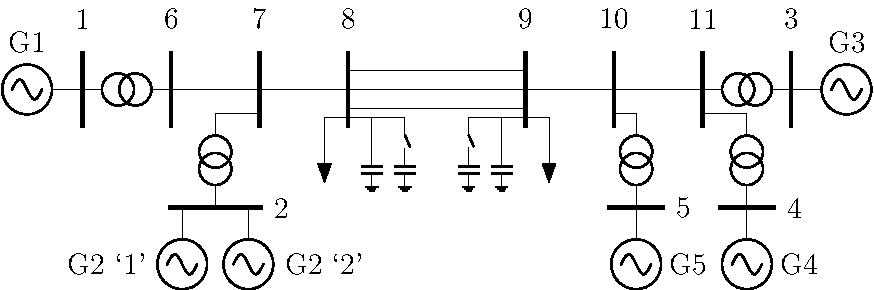
\includegraphics[width=\linewidth]{../../../TEX/models/sixMachine/sixMachine}
	\caption{Two Area Six Machine System.}
	\label{fig: six machine}
\end{figure}

\paragraph{Results:} 
Definite time controller appears to function as desired.
PSLTDSim could be used for capacitor switching coordination.
When load and generation ramps together odd frequency `blips' occur when shunts are switched.
When load is not ramped with generation, AGC forces generator 3 to a very low power generation point.


\newcommand{\caseName}{def}
\newcommand{\scrunch}{\vspace{-.8em}}
\pagebreak
\paragraph{CASE 1: Voltage control on shunts only. Generation and Load Ramp} \ \\
\renewcommand{\caseName}{sixMachineWindramp1}
\scrunch
\includegraphics[width=\linewidth]{figures/\caseName sysShuntV}
\scrunch
\includegraphics[width=\linewidth]{figures/\caseName MVarflow8to9}
\scrunch
\includegraphics[width=\linewidth]{figures/\caseName sysShuntMVAR}
\scrunch
\includegraphics[width=\linewidth]{figures/\caseName sysPePmLoad2}

\pagebreak
\paragraph{CASE 1: Voltage and Qbr control on shunts. Generation and Load Ramp} \ \\
\renewcommand{\caseName}{sixMachineWindramp2}
\scrunch
\includegraphics[width=\linewidth]{figures/\caseName sysShuntV}
\scrunch
\includegraphics[width=\linewidth]{figures/\caseName MVarflow8to9}
\scrunch
\includegraphics[width=\linewidth]{figures/\caseName sysShuntMVAR}
\scrunch
\includegraphics[width=\linewidth]{figures/\caseName sysPePmLoad2}

\pagebreak
\paragraph{CASE 3: Voltage control on shunts only. Generation Ramp only} \ \\
\renewcommand{\caseName}{sixMachineWindramp3}
\scrunch
\includegraphics[width=\linewidth]{figures/\caseName sysShuntV}
\scrunch
\includegraphics[width=\linewidth]{figures/\caseName MVarflow8to9}
\scrunch
\includegraphics[width=\linewidth]{figures/\caseName sysShuntMVAR}
\scrunch
\includegraphics[width=\linewidth]{figures/\caseName sysPePmLoad2}

\end{document}